\documentclass{report}
\usepackage{enumerate}
\usepackage{amsmath}
\usepackage{multirow}
\usepackage{amsfonts}
\usepackage{graphicx}
\usepackage{tikz}
\usetikzlibrary{fadings}
\newcommand{\xmark}{$\times$}
\pgfkeys{%
/piechartthreed/.cd,
scale/.code                =  {\def\piechartthreedscale{#1}},
mix color/.code            =  {\def\piechartthreedmixcolor{#1}},
background color/.code     =  {\def\piechartthreedbackcolor{#1}},
name/.code                 =  {\def\piechartthreedname{#1}}}

 \newcommand\piechartthreed[2][]{% 
   \pgfkeys{/piechartthreed/.cd,
     scale            = 1,
     mix color        = gray,
     background color = white,
     name             = pc} 
  \pgfqkeys{/piechartthreed}{#1}
  \begin{scope}[scale=\piechartthreedscale] 
  \begin{scope}[xscale=5,yscale=3] 
     \path[preaction={fill=black,opacity=.8,
         path fading=circle with fuzzy edge 20 percent,
         transform canvas={yshift=-15mm*\piechartthreedscale}}] (0,0) circle (1cm);
    \fill[gray](0,0) circle (0.5cm);  
     \path[preaction={fill=\piechartthreedbackcolor,opacity=.8,
          path fading=circle with fuzzy edge 20 percent,
          transform canvas={yshift=-10mm*\piechartthreedscale}}] (0,0) circle (0.5cm);
     \pgfmathsetmacro\totan{0} 
     \global\let\totan\totan 
     \pgfmathsetmacro\bottoman{180} \global\let\bottoman\bottoman 
     \pgfmathsetmacro\toptoman{0}   \global\let\toptoman\toptoman 
     \begin{scope}[draw=black,thin]
     \foreach \an/\col [count=\xi] in {#2}{%
     \def\space{ } 
        \coordinate (\piechartthreedname\space\xi) at (\totan+\an/2:0.75cm); 
        \ifdim 180pt>\totan pt 
         \ifdim 0pt=\toptoman pt
            \shadedraw[left color=\col!20!\piechartthreedmixcolor,
                       right color=\col!5!\piechartthreedmixcolor,
                       draw=black,very thin] (0:.5cm) -- ++(0,-3mm) arc (0:\totan+\an:.5cm) 
                                                       -- ++(0,3mm)  arc (\totan+\an:0:.5cm);
            \pgfmathsetmacro\toptoman{180} 
            \global\let\toptoman\toptoman         
            \else
            \shadedraw[left color=\col!20!\piechartthreedmixcolor,
                       right color=\col!5!\piechartthreedmixcolor,
                       draw=black,very thin](\totan:.5cm)-- ++(0,-3mm) arc(\totan:\totan+\an:.5cm)
                                                        -- ++(0,3mm)  arc(\totan+\an:\totan:.5cm); 
          \fi
        \fi   
        \fill[\col!20!gray,draw=black] (\totan:0.5cm)--(\totan:1cm)  arc(\totan:\totan+\an:1cm)
                                     --(\totan+\an:0.5cm) arc(\totan+\an:\totan :0.5cm);     
       \pgfmathsetmacro\finan{\totan+\an}
       \ifdim 180pt<\finan pt 
         \ifdim 180pt=\bottoman pt
            \shadedraw[left color=\col!20!\piechartthreedmixcolor,
                       right color=\col!5!\piechartthreedmixcolor,
                       draw=black,very thin] (180:1cm) -- ++(0,-3mm) arc (180:\totan+\an:1cm) 
                                                       -- ++(0,3mm)  arc (\totan+\an:180:1cm);
            \pgfmathsetmacro\bottoman{0}
            \global\let\bottoman\bottoman
            \else
            \shadedraw[left color=\col!20!\piechartthreedmixcolor,
                       right color=\col!5!\piechartthreedmixcolor,
                       draw=black,very thin](\totan:1cm)-- ++(0,-3mm) arc(\totan:\totan+\an:1cm)
                                                        -- ++(0,3mm)  arc(\totan+\an:\totan:1cm); 
          \fi
        \fi
        \pgfmathsetmacro\totan{\totan+\an}  \global\let\totan\totan 
       } 
    \end{scope}
    \draw[thin,black](0,0) circle (0.5cm);
   \end{scope}  
\end{scope}
}
\begin{document}
\tableofcontents
\listoffigures
\listoftables
\chapter{A summary of the approaches}
~~In the proposed system by wu et all  we find a task scheduling algorithm by based on Qos driven in cloud computing. One of the challenges posed by cloud applications is Quality-of-Service (QoS) management, which is the problem of allocating resources to the application to guarantee a service level along dimensions such as performance, availability and reliability. In their paper, they have proposed an algorithm to compute priority based on special attribute of task. Moreover it sorts the tasks according to their priority .As the performance is the main issue the algorithm calculates the completion of each task .Then it schedules each task according to priority as well as completion time.\cite{Wu}\\\\
\verb|  |Jhang et all proposed a system that works on the  genetic algorithm. The proposed system  considers users satisfaction and the availability of virtual machines. The genetic function in the system iterates to find the best possible task schedule.\cite{Jhang}\\\\
\verb|  |The system proposed by M. paul is a dynamic task scheduling. The paper is mainly on horizontal load balancing. In this paper the author used a quite innovative way ,they considered task scheduling problem as an assignment problem in mathematics. Then after conversion they go for optimal solution using lexi search approach.\cite{Paul}\\\\
\verb|  |S.Bitam find an improvement in job scheduling in clod environment. In their paper they have used bee\verb|'|s life algorithm to find the optimal solution. They have also provided the proof that bee\verb|'|s life algorithm provides a better result then genetic algorithm. For performance evaluation they have used makespan as their main objective.\cite{Bitam}\\\\
\verb|  |S.Behzad et all proposed a system that has a queue base job scheduling algorithm. They have also compared that their proposed system  with First come first serve(FCFS),Robin round(RR),Shortest job first(SJF) approaches. By the simulation result they have proved that queue based job scheduling provided a far better result then these.\cite{Behzad} \\\\
\verb|  |In the paper of Dumitrescu et al. we find a quite different  approach , job scheduling through bin packaging problem. For the detection of equilibrium  they have used evolutionary approach. They showed that for a large number of players in cloud aumann equilibrium provides a better result than nash equilibrium.\cite{Dumitrescu}\\\\
\verb|  |Green computing has become a new paradigm in cloud computing and Ahmed et all provides a good solution of that problem. They  have proposed a system considering energy  consumption as their main objective. Moreover they have converted energy aware task allocation problem into a job scheduling problem.\cite{Ahmed}\\\\
\verb|  |The proposed system of Ge song et all is for Hadoop architecture .In their solution scheduling is divided into two levels. In first level of Hadoop job scheduling , bid model is used to find the job  to execute .At second level of Hadoop task scheduling game Hungarian method is used. In this step the at first the job scheduling problem is converted into an assignment problem then it is solved using Hungarian method.\cite{Ge}\\\\
\verb|  |Pillai et all proposed a system using principal of coalition formation and uncertainty principal of  game theory. Authors used coalition formation for resource allocation  and then analyzed their resources by various parameters like allocation time, resource wastage etc.\cite{Pillai}\\\\
\verb|  |Lie et all proposed a system  for reality based job scheduling using non cooperative game model. The system ensures hair resource allocation for all users in cloud. The final solution is provided using nash equilibrium for game theory.\cite{Li}\\\\
\verb|  |Abdeyazdan et al. proposed a task graph pre-scheduling algorithm. The algorithm is  for a network of homogeneous processors using Nash Equilibrium concepts of game theory. Their main objective is  the reduction of the idle time of the system .So that there is an overall a increase in the throughput.\cite{Abdeyazdan}\\\\
\chapter{Comparison}
The authors have used several criteria for evaluating the papers or proposed systems. The papers authors have covered has met some of this criteria. But none of the papers met all the criteria\verb|'|s.
A description of the evaluation criteria are:
\\
\begin{enumerate}[A.]

\item \textbf{Makespan:} By makespan authors have  meant the time spent by the system from the beginning of  first task to the end of the last task of the job. It has been considered that makespan is one of the most important measurement of scheduling algorithms.
\item \textbf{Fairness:} Fairness  measures are normally used in network engineering. In network engineering fairness means whether  users are receiving a fair share of resource .Fair share  of resource plays a significant role in scheduling of jobs as the fair resource allocation reflects users satisfaction.
\item \textbf{Optimization:} By optimization the authors meant the process by which  cost effective and highest achievable performance under given constraint can be achieved. Optimization also means the maximization of the desired and the minimization of the undesired factors.
\item \textbf{Energy Consumption:} Green computing has been a new paradigm in cloud computing and a few system or algorithms are concern about the energy consumption. By energy consumption factor authors means the amount of energy consumed by the system. As  low the energy consumption as good the system is.
\item \textbf{Load balancing:} It is a computer networking method may be defines as the distribution of work loads among multiple computer resources. By proper load balancing a system can significantly reduce energy consumption.
\item \textbf{Deadline:} Generally deadline means the final time by which something has to be completed. In this paper authors also meant something like this.In cloud computing meeting the users requirements QoS\footnote{Quality of Service} and also SLA\footnote{Service Level Agreement} within the specified time comes under deadline.
\item \textbf{Execution time:} It is the time spent by the system to execute a task. In cloud computing scenario it can be considered the time taken by the system to process users request as well as give services. To increase performance of a system one has to take  execution time as their main objective.
\end{enumerate}
\begin{figure}

 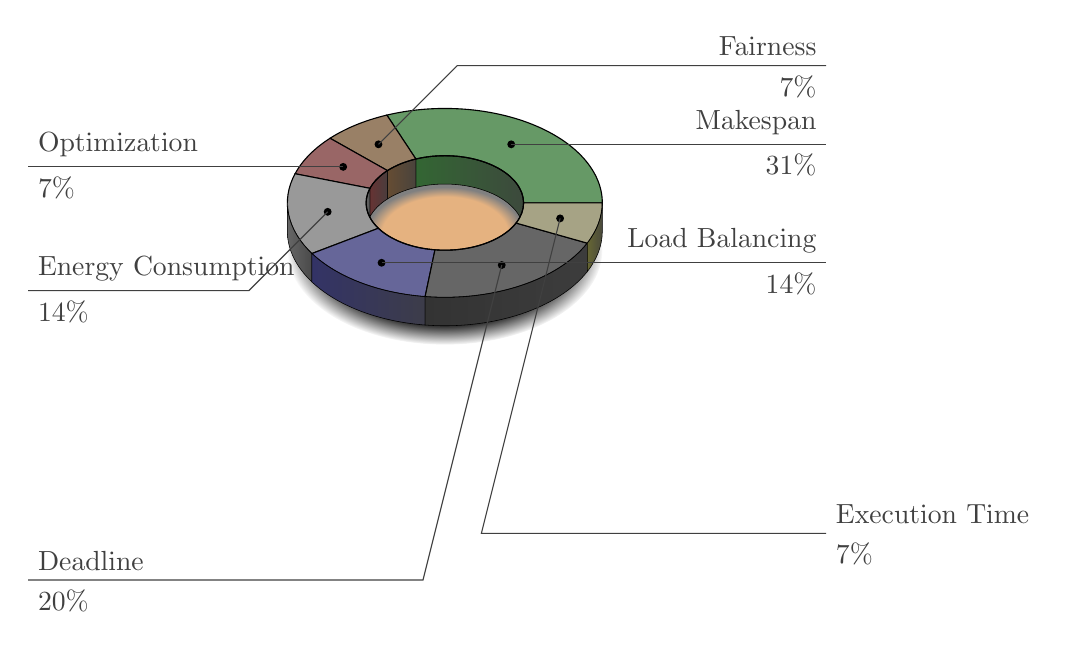
\begin{tikzpicture}
   \piechartthreed[scale=0.4,
                   background color=orange!50,
                   mix color= darkgray]
                   {111.6/green,25.2/orange,25.2/red,50.4/white,50.4/blue,72/black,25.2/yellow}
   \foreach \i in {1,...,7} { \fill (pc \i) circle (.5mm);}
   \draw[darkgray] (pc 1)  -- ++(4,0) coordinate (s1) node[anchor=south east] {Makespan}
                                                      node[anchor=north east] {31\%};
   
   \draw[darkgray] (pc 2)  -- ++(1,1) coordinate (s2) -- (s2 -| s1) node[anchor=south east] {Fairness}
                                                      node[anchor=north east] {7\%}; 
   \draw[darkgray] (pc 3)  -- ++(-4,0) coordinate (s3) node[anchor=south west] {Optimization}
                                                      node[anchor=north west] {7\%};
   \draw[darkgray] (pc 4)  -- ++(-1,-1) coordinate (s4) --(s4 -| s3) node[anchor=south west] {Energy Consumption}
                                                      node[anchor=north west] {14\%};
      \draw[darkgray] (pc 5)  -- (pc 5 -| s1) coordinate (s5) --(s5 -| s1) node[anchor=south east] {Load Balancing}
                                                     node[anchor=north east] {14\%};                                                    
   \draw[darkgray] (pc 6)  -- ++(-1,-4) coordinate (s6) --(s6 -| s3) node[anchor=south west] {Deadline}
                                                     node[anchor=north west] {20\%};                                                   
   \draw[darkgray] (pc 7)  -- ++(-1,-4) coordinate (s7) --(s7 -| s1) node[anchor=south west] {Execution Time}
                                                     node[anchor=north west] {7\%};                                                  
                                                
 \end{tikzpicture}
 \caption{Parameters covered by approaches}
 
\end{figure}


\begin{table}[]
\centering
        \small
        \setlength\tabcolsep{1pt}
        
\rotatebox{90}{

\begin{tabular}{|c|c|c|c|c|c|c|c|c|}
\hline
 Papers Parameters&  Makespan & Fairness & Optimization &\shortstack[l]{ Energy\\Consumption} & \shortstack[r]{Execution\\Time} & \shortstack[l]{Load\\Balancing} & \shortstack[l]{User\\Satisfaction} & Deadline \\ \hline
 \shortstack[l]{\\A game-theory approach\\ for job scheduling \\ in networked manufacturing} & \checkmark & \xmark &\xmark  & \xmark &\xmark  & \xmark & \xmark & \xmark \\ \hline
\shortstack[l]{\\Non-cooperative games \\on multi-dimensional\\ resource allocation} & \xmark & \xmark & \xmark & \xmark & \xmark & \checkmark & \xmark & \xmark \\ \hline
\shortstack[l]{\\A game-theoretic method of\\ fair resource allocation\\ for cloud computing services}& \xmark & \checkmark & \checkmark & \xmark &\xmark  & \xmark & \xmark & \xmark \\ \hline
\shortstack[l]{\\Job Scheduling Model for \\Cloud Computing Based on\\ Multi-Objective Genetic Algorithm}& \xmark &\xmark  & \xmark & \checkmark & \xmark & \xmark &\xmark  & \xmark \\ \hline
\shortstack[l]{\\Sla-based cooperative super\\ scheduling algorithms for\\ computational grids} & \xmark & \xmark & \xmark & \xmark &\xmark  & \xmark &\xmark  &\checkmark  \\ \hline
\shortstack[l]{\\A Task Scheduling Algorithm\\ based on QoS-Driven\\ in Cloud Computing} & \xmark & \xmark & \xmark & \xmark &\checkmark  & \checkmark & \xmark & \xmark \\ \hline
\shortstack[l]{\\The Study of Genetic\\ Algorithm-based Task\\ Scheduling for Cloud Computing} & \xmark & \xmark & \xmark & \xmark &\xmark  & \xmark & \checkmark & \xmark \\ \hline
\shortstack[l]{\\Dynamic job scheduling\\ in cloud computing\\ based on horizontal load balancing} &\xmark  &\xmark  &\xmark  & \xmark & \xmark & \checkmark &\xmark  & \xmark \\ \hline
\shortstack[l]{\\Bees Life Algorithm for \\job scheduling in\\ cloud computing} & \checkmark & \xmark & \xmark & \xmark & \xmark & \xmark & \xmark & \xmark \\ \hline
\shortstack[l]{\\Queue based Job Scheduling \\algorithm for Cloud computing} & \xmark & \xmark & \xmark & \xmark & \checkmark & \xmark & \xmark & \xmark \\ \hline
\shortstack[l]{\\Using Game Theory for\\ Scheduling Tasks on\\ Multi-Core Processors\\ for Simultaneous
Optimization \\of Performance and Energy} &\checkmark  & \xmark & \xmark & \checkmark & \xmark & \xmark & \xmark & \xmark \\ \hline
\shortstack[l]{\\A Non-Cooperative Game \\Model for Reliability-Based\\ Task Scheduling in Cloud
Computing} & \xmark & \checkmark & \xmark & \xmark & \xmark & \xmark & \xmark & \xmark \\ \hline
\end{tabular}
}
\caption{Scheduling parameters considered by existing algorithms}
\end{table}
\chapter{Findings}
 In the papers  authors have found some interesting breakthrough in the field of cloud computing>findings like the inter relation of parameters will help the enthusiasts in this field to choose the correct parameter to cover.Findings are briefly explained as follows:
 \begin{enumerate}
 \item \textbf{	Aumann equilibrium supremacy:} For a large number of player in the cloud the aumann equilibrium provides a far more optimized scheduling then nash equilibrium.
\item \textbf{Final Solution point:} For non co-operative game theory Nash equilibrium is the final solution point. There is nothing like final solution point in Co-operative game theory .The authors have recommended some of techniques like Pareto optimality, Pareto Efficiency, co-ordination failure for  finding solution in the scenario of co operative game theory.
\item \textbf{Parameters inter relation:} The parameters authors used to compare the papers are inter related .That means if  one system covers one parameter multiple parameter may be covered automatically. Like when fairness and deadline parameter  constraints are met user satisfaction will be automatically met. As fairness will ensure fair resource allocation for each job and deadline will execute the users job  at due time. So customer satisfaction will be met. If any system taken care of the execution time constraint that will reduce makespan and thereby reduces  the total energy consumption of the system.
\item \textbf{Load balancing:} Load  balancing provides  better result in terms of reduction of the total energy consumption of the system.

 \end{enumerate}
 
\chapter{Drawback}
It seems the paper lacks clarification on some topics.If the authors make their position more transparent and authentic that would be excellent.\\\\
\verb|  |In that paper authors, have simply state what the authors\footnote{The authors of the papers they have covered} of the paper they have covered has done or their main objective. But they have not provided any type of proof or cause why the proposed system is bad or good.\\
\verb|  |Authors have selected many parameters for comparison of approaches but they have not provided any reason why they have selected those parameters.\\
\verb|  |In the paper The authors have stated that finish time is the main drawback for algorithms but they have not provided any time of cause or proof supporting their statement. \\
\verb|  |Later they have quoted a paper that have stated that further improvement is possible beyond nash equilibrium using Particle swarm optimization(PSO), Ant colony optimization(ACO), Simulated Annealing(SA). But there are not reference of that paper for readers. \\
\verb|  |The authors also recommend some further work in this field. Like most of the paper covered in this paper are covering one or two parameters so a solution covering all the parameters may be a considered a good task and different approach has different drawbacks so a combination of all the positive traits may also be considered an excellent task in this field. If there were any definite list of drawbacks of parameter authors provided that would be easy for enthusiast for future work in this field.
\chapter{Conclusion}
In cloud environment job scheduling is considered an important task.There are many job scheduling algorithm for cloud is available with different positive traits and feature.A comparison  or survey in this field is necessary to find the scope or future direction in this field.In that context the paper is very useful and informative for the enthusiasts in this field.
\bibliographystyle{plain}
\bibliography{report}
\end{document}